\documentclass[25pt, margin=0mm, innermargin=15mm, blockverticalspace=15mm, colspace=15mm, subcolspace=8mm]{beamer}
\geometry{paperwidth=40cm,paperheight=181cm}

% to stretch boxes over whole paper with custor paper size
\makeatletter
\setlength{\TP@visibletextwidth}{\textwidth-2\TP@innermargin}
\setlength{\TP@visibletextheight}{\textheight-2\TP@innermargin}
\makeatother

\usepackage{fix-cm}  
\makeatletter
\newcommand\HUGE{\@setfontsize\Huge{80}{90}}
\makeatother

\usepackage{wrapfig}

\definecolor{textcolor}{HTML}{000000}
\definecolor{colorOne}{HTML}{4cbf5d}
\definecolor{colorTwo}{HTML}{dddddd}
\definecolor{colorThree}{HTML}{12343a}

\hypersetup
{
    pdfauthor={Y. Chemin},
    pdfsubject={},
    pdftitle={Open Monitoring Systems Working Group},
    pdfkeywords={}
}

\graphicspath{{images/}{logos/}}

\usepackage[percent]{overpic}
\usepackage{tikz}
\tikzset{
  every overlay node/.style={
    draw=white,fill=white,rounded corners,anchor=north west,
  },
}
% Usage:
% \tikzoverlay at (-1cm,-5cm) {content};
% or
% \tikzoverlay[text width=5cm] at (-1cm,-5cm) {content};
\def\tikzoverlay{%
   \tikz[baseline,overlay]\node[every overlay node]
}%

\begin{document}


\tikzoverlay at (-1.2cm,1.2cm) {
\begin{tikzpicture}
   % NODES
   \node (r0) at (40.0,  0.0) {}; % root
   \node (s0) at (20.0, -160.0) {}; % extreme
   \node (s1) at (40.0, -180.0) {}; % extreme

   % DRAW TREE
   \fill[fill=colorThree,colorThree] (r0.center)--(s0.center)--(s1.center);
   \path[draw] (r0)--(s0);
   \path[draw] (s0)--(s1);
   \path[draw] (s1)--(r0);

   % NODES
   \node (r1) at (-0.1,  -100.5) {}; % root
   \node (s10) at (40.3, -220.0) {}; % extreme
   \node (s11) at (50.0, -165.0) {}; % extreme

   % DRAW TREE
   \fill[fill=colorOne,colorOne] (r1.center)--(s10.center)--(s11.center);
   \path[draw] (r1)--(s10);
   \path[draw] (s10)--(s11);
   \path[draw] (s11)--(r1);

\end{tikzpicture}
}

\tikzoverlay at (5cm,-35cm){
\begin{tikzpicture}[overlay]
\node at (current page.south west) [above right, inner sep=0,outer sep=0]
	{
\includegraphics[height=25cm]{osgeo.pdf}};
\end{tikzpicture}
}

\tikzoverlay at (5cm,-55cm){
\begin{tikzpicture}[overlay]
	\node at (current page.south west) [above right,text width=40cm,align=left] {\HUGE{\textbf{\color{colorThree}Open \\Monitoring \\Systems \\Working Group}}};
\end{tikzpicture}
}

\tikzoverlay at (5cm,-70cm){
\begin{tikzpicture}[overlay]
	\node at (current page.south west) [above right,text width=40cm,align=left] {\Huge{\color{colorThree}https://wiki.osgeo.org/wiki/Open\_Monitoring\_Systems\_Working\_Group}};
\end{tikzpicture}
}

\tikzoverlay at (-1.2cm,-181cm){
\begin{tikzpicture}[overlay]
\node at (current page.south west) [above right, inner sep=0,outer sep=0]
	{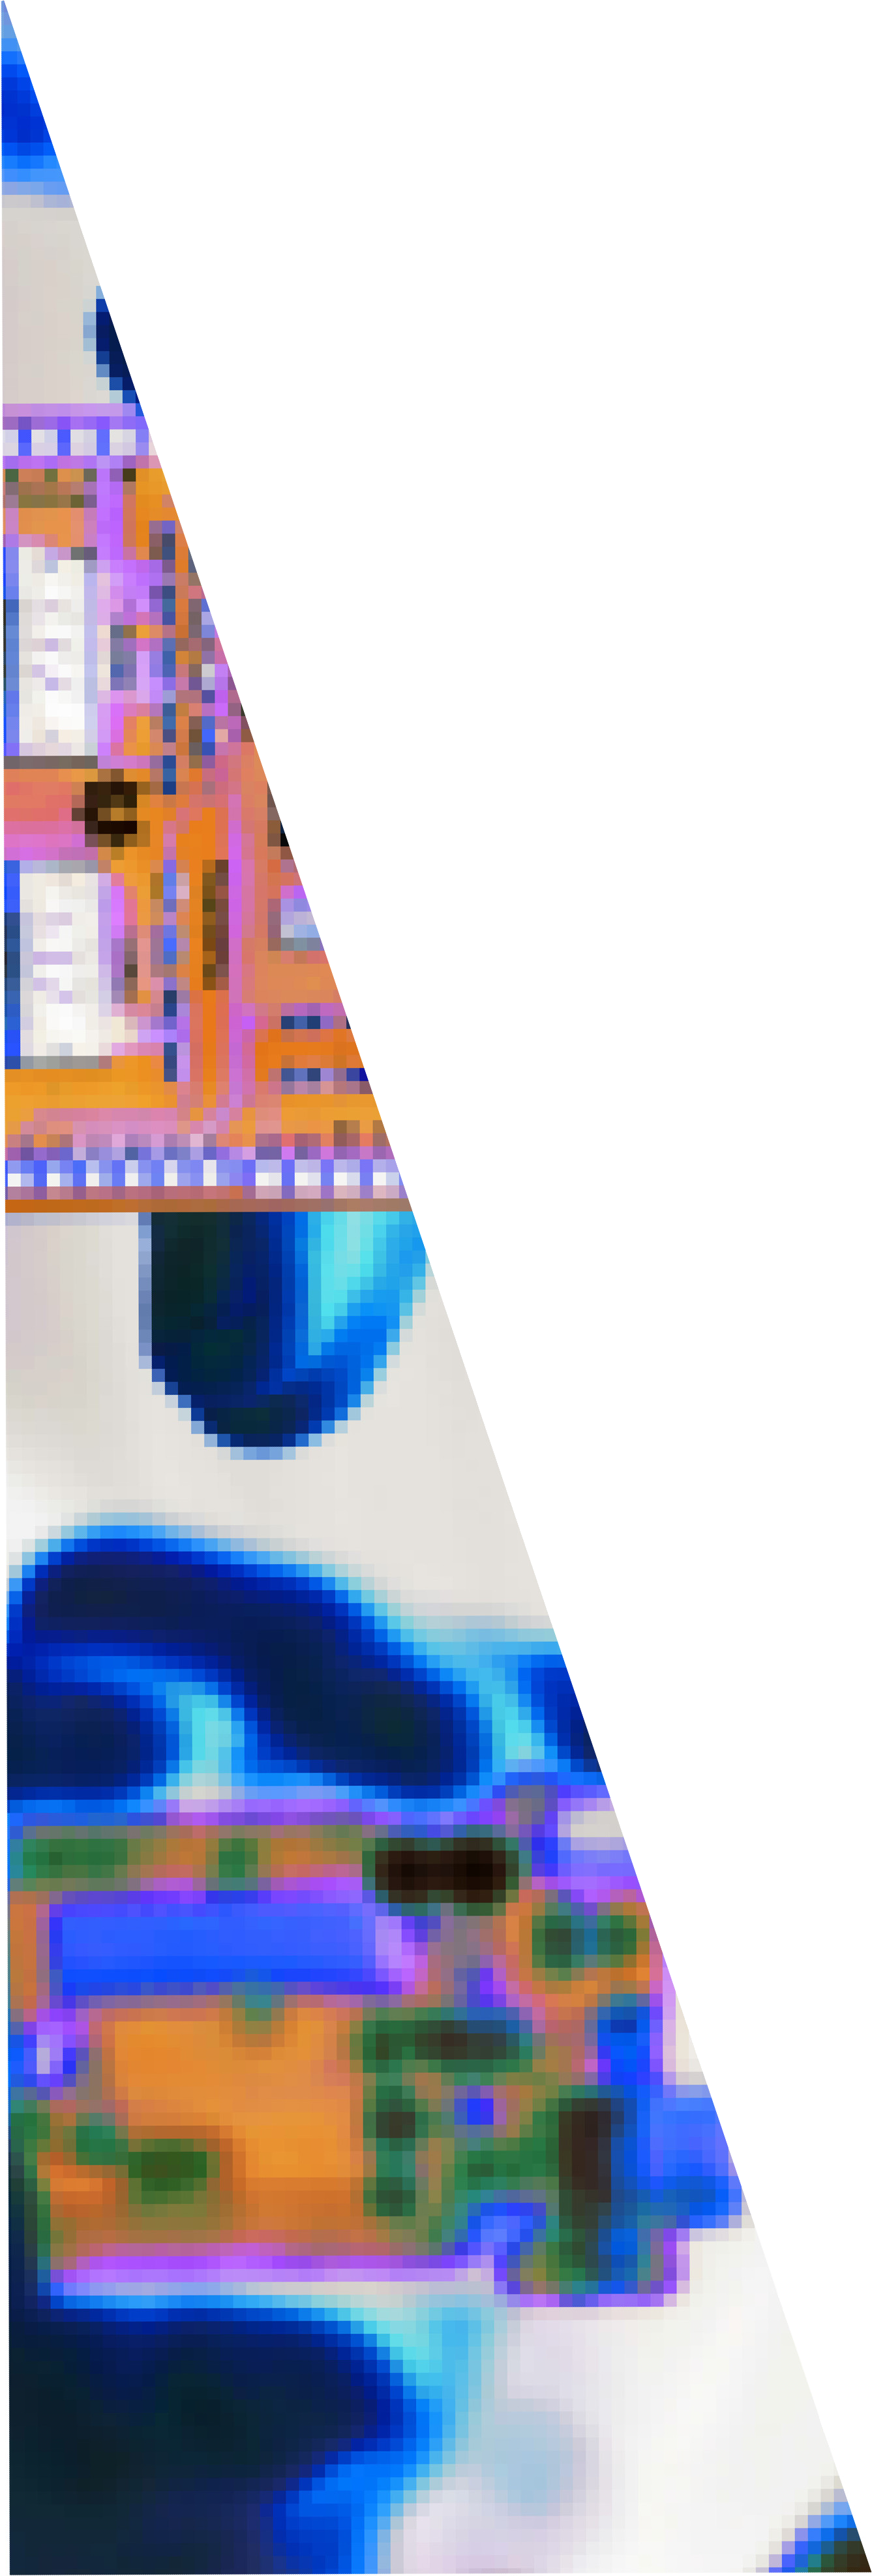
\includegraphics[height=81.5cm]{elec2.png}};
\end{tikzpicture}
}

\tikzoverlay at (-1.2cm,1.2cm) {
\begin{tikzpicture}[overlay]
	\draw [draw=green,thick] (0,-100) (20.0,-160.0);
\end{tikzpicture}
}
%%%%%%%%%%%%%%%%%%%%%%%%%%%%%%%%%%%%%%%%%%%%%%%%%%%%%%%%%%%%%%%%%%%%%%%%%%%%%%%%

\end{document}
